
\section{計畫執行內容}

\subsection{教學實踐研究計畫動機}
\label{sec:introduction}

\subsubsection{教學問題脈絡}

隨著人工智慧技術的普及,程式設計能力已成為21世紀公民的基本素養,
運算思維(Computational Thinking)更被視為跨領域問題解決的核心能力\cite{wing2006computational}。
本校通識教育中心開設之「初級程式設計-Python」課程,參考哈佛大學CS50P課程設計\cite{cs50p2024},
旨在培養非資訊科系學生的運算思維與程式設計能力。
然而,教學實踐中面臨三大核心挑戰:

\textbf{挑戰一:學習困難與高挫折率}

113學年度課程資料顯示,62\%學生反映初期學習困難,期中考僅47\%及格,且僅31\%學生能獨立完成期末專題。
非資訊背景學生在學習程式設計時面臨多重障礙,包括抽象概念理解困難、語法錯誤頻繁、
缺乏問題分解能力等\cite{guzdial2015learner,qian2017misconceptions}。

\textbf{挑戰二:生成式AI帶來的認知卸載危機}

研究顯示,OpenAI Codex等AI程式碼生成工具能以約78\%的準確率解決入門程式設計問題\cite{finnieansley2022robots},
而透過自然語言提示(prompt engineering)與ChatGPT、GitHub Copilot等工具互動,
學生可快速獲得程式碼建議\cite{denny2023conversing},
為程式設計教育帶來前所未有的機會與挑戰\cite{becker2023programming}。
然而,學生過度依賴AI可能導致「認知卸載」(cognitive offloading),即將思考過程外包給AI,
而未真正理解程式邏輯\cite{kazemitabaar2023studying}。
研究顯示,學生傾向於直接接受AI生成的程式碼而不加驗證,即使程式碼包含錯誤也難以察覺\cite{prather2024weird}。
此外,AI工具在進階程式設計問題(如CS2資料結構與演算法)上同樣表現優異,能超越多數學生\cite{finnieansley2023exam},
這使得學生更容易產生依賴心理。

\textbf{挑戰三:傳統教學方法的侷限}

傳統的「講述-練習」教學模式難以有效支持學生建立自主學習能力。
教師難以即時診斷每位學生的學習困難,也無法提供個別化的學習支持。
此外,國內針對非資訊科系學生的程式設計教學研究也指出,
單向講授模式不利於培養學生的運算思維與問題解決能力\cite{lin2021teaching,lai2020analysis}。

\subsubsection{傳統教學方法說明}

過去本課程採用以下教學方法:

\begin{enumerate}
\item \textbf{講述法為主}:教師透過投影片講解程式概念與語法,學生被動接收知識。
\item \textbf{範例示範}:教師示範程式碼撰寫過程,學生模仿練習。
\item \textbf{課後作業}:指派固定題目供學生練習,但缺乏即時回饋機制。
\item \textbf{AI工具使用方式}:允許學生自由使用ChatGPT等工具,但未提供使用指引或限制。
\end{enumerate}

此模式的主要問題:
\begin{itemize}
\item 學生缺乏主動探索與問題解決的機會
\item 無法培養自我調節學習能力
\item AI工具使用缺乏教學設計,導致過度依賴
\item 評量方式難以區分學生真實能力與AI協助程度
\end{itemize}

\subsubsection{改進方向與預期效益}

有鑑於此,本研究提出「AI鷹架漸退式教學模式」(AI Scaffolding Fading Model),
結合自我調節學習理論(Self-Regulated Learning, SRL)\cite{zimmerman2002becoming,azevedo2019using}
與問題導向學習(Problem-Based Learning, PBL)\cite{savery2006overview,hmelo2004problem},
將AI從「答案提供者」轉變為「學習鷹架」。
此教學設計參考認知學徒制(Cognitive Apprenticeship)中的鷹架理論\cite{collins1989cognitive,wood1976role},
透過逐步減少外部支持,促進學生建立內在學習策略與自主學習能力\cite{jarvela2015enhancing}。

\textbf{研究創新性}:有別於現有研究多聚焦於AI工具對學習成效的影響\cite{kazemitabaar2023studying,kazemitabaar2024codeaid},
本研究首次提出系統化的AI鷹架漸退機制,並結合學習歷程資料分析,
探討如何透過教學設計引導學生從「AI依賴」轉向「AI協作」,最終達到「自主學習」(如圖\ref{fig:framework}所示)。

\begin{figure}[htbp]
  \centering
  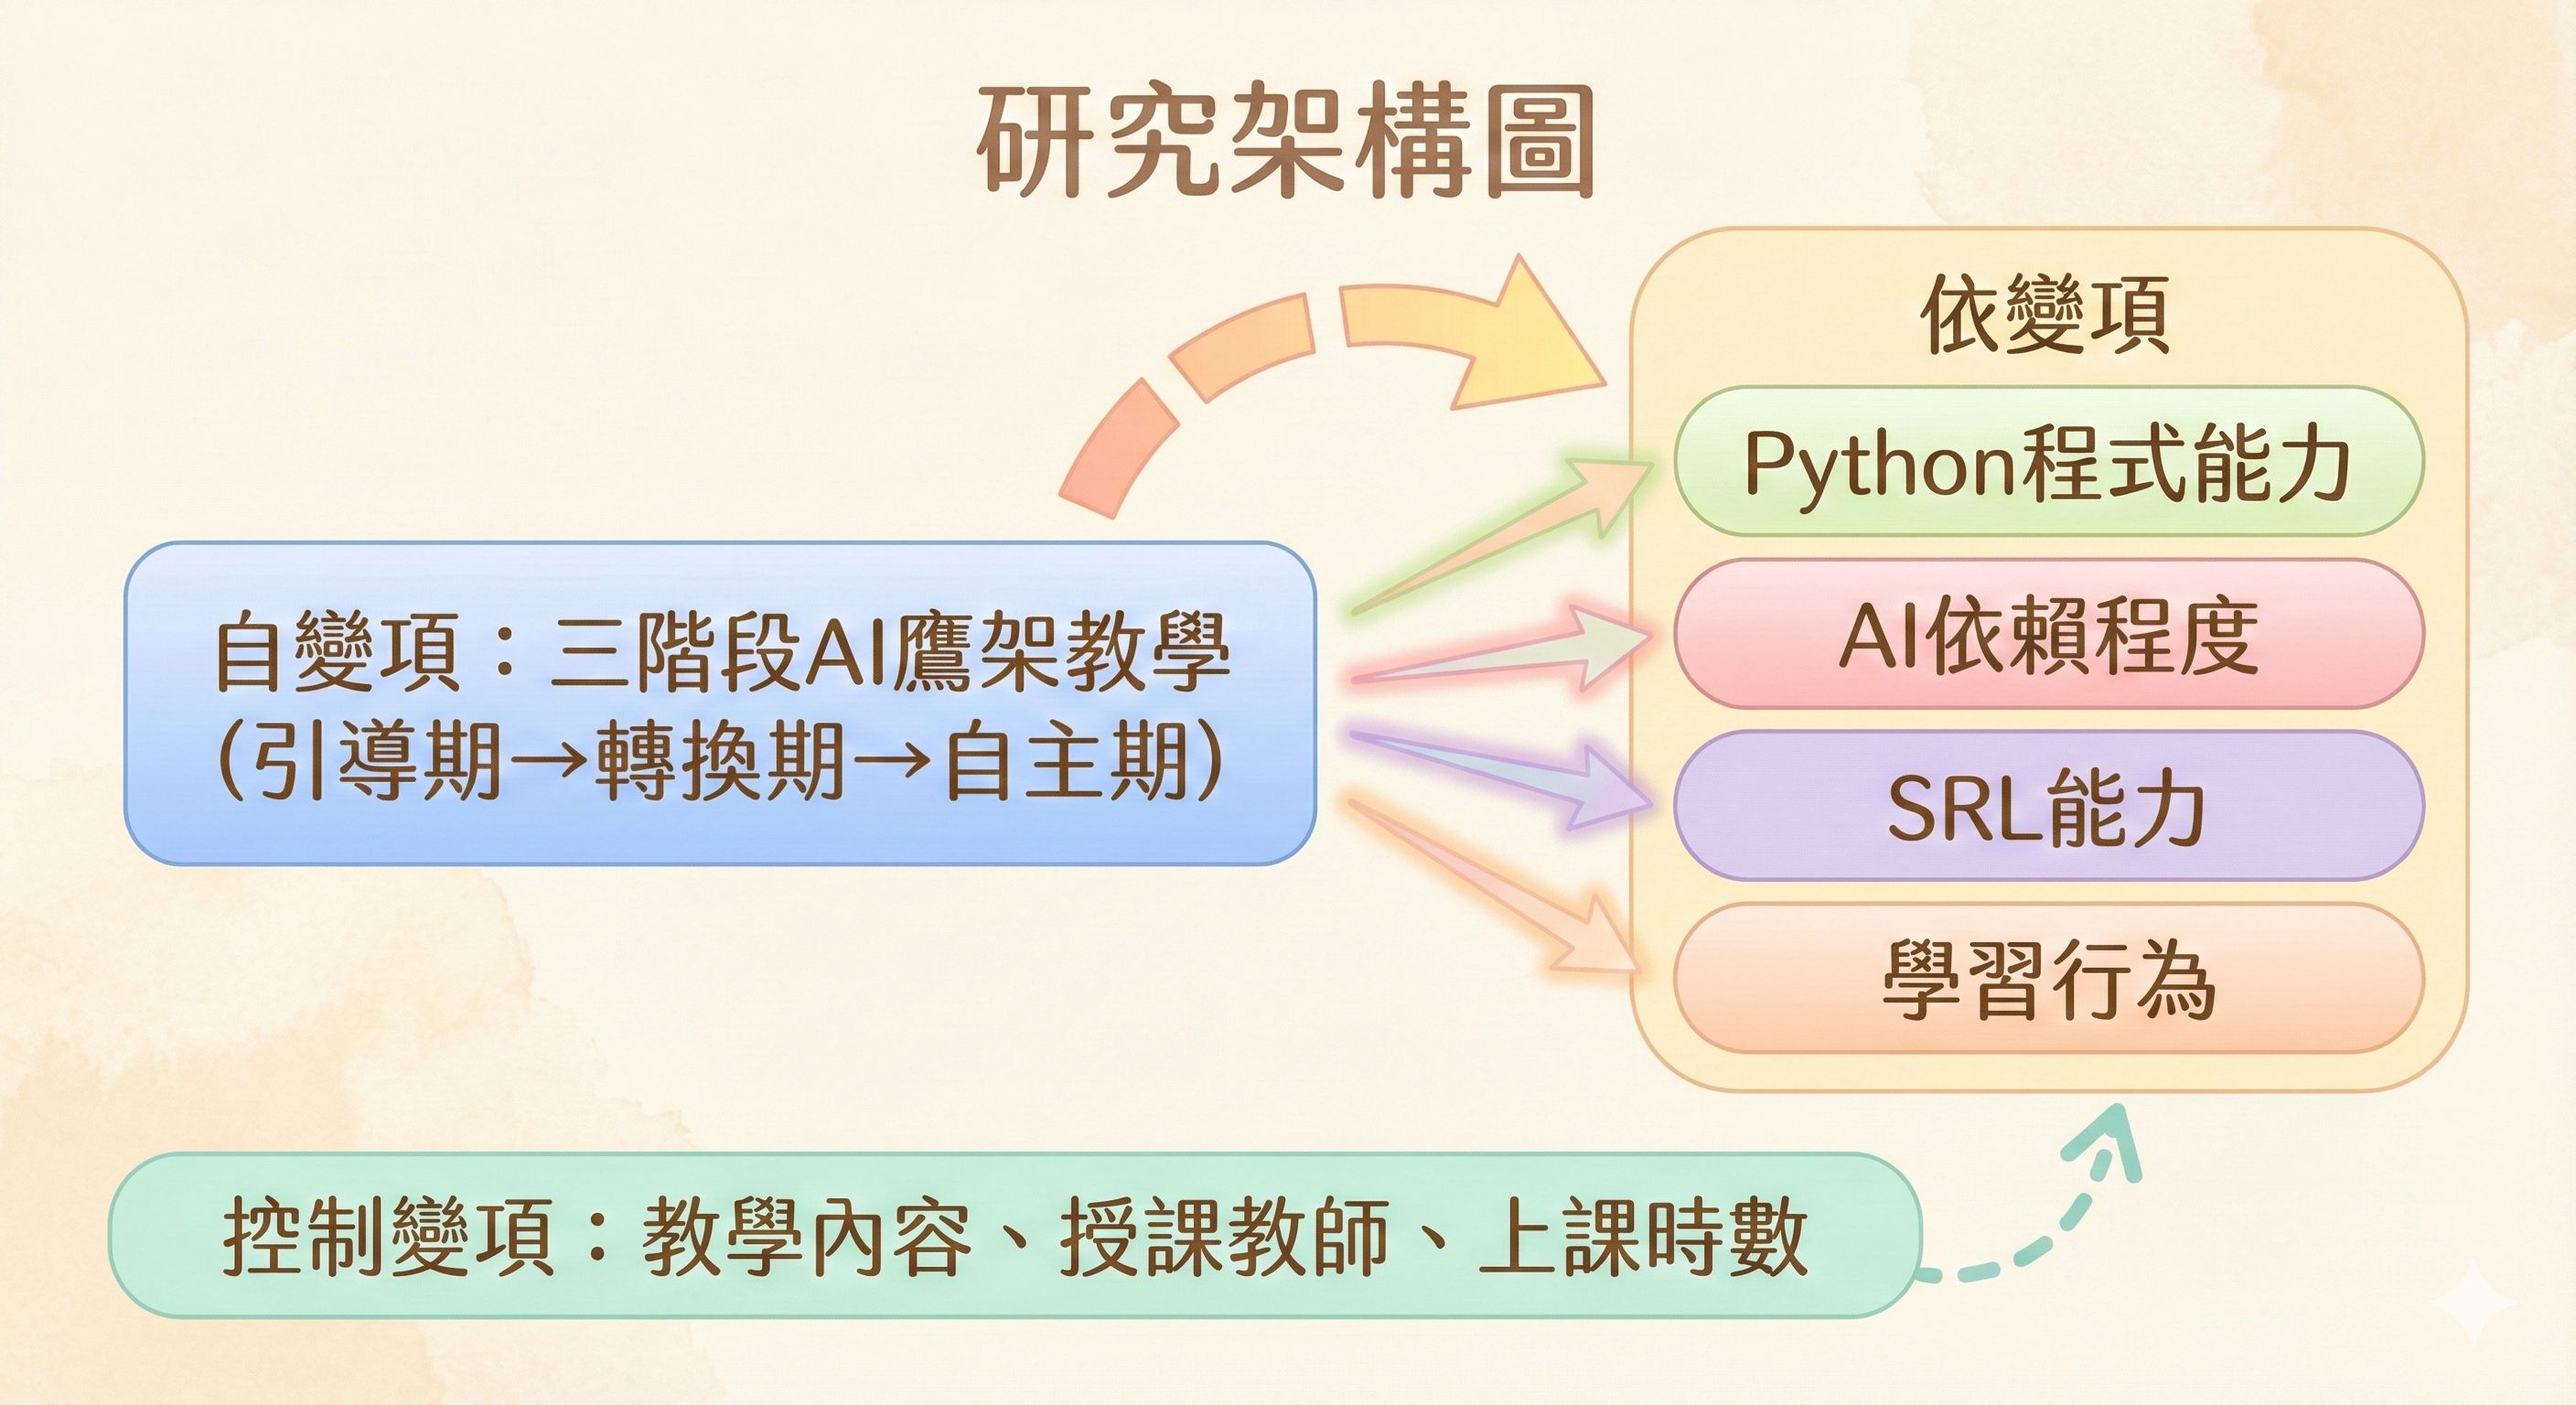
\includegraphics[width=0.85\linewidth]{framework.png}
  \caption{研究架構圖}
  \label{fig:framework}
\end{figure}

\textbf{核心理念}:透過三階段AI鷹架漸退設計:
\begin{enumerate}
\item \textbf{引導期}(1-6週):高度結構化AI提示,引導學生思考
\item \textbf{轉換期}(7-12週):部分鷹架移除,鼓勵學生先嘗試
\item \textbf{自主期}(13-18週):最小化AI介入,學生主導學習
\end{enumerate}

\textbf{預期效益}:
\begin{itemize}
\item 提升學生程式設計學習成效與自我效能,促進內在學習動機\cite{ryan2000selfdetermination}
\item 降低AI過度依賴,培養自我調節學習能力
\item 發展有效的AI輔助教學模式,可推廣至其他課程
\item 探索AI工具在教育中的負責任使用方式\cite{dignum2019responsible}
\end{itemize}

具體而言,本研究以「先思考、後求助、再驗證」為核心原則,
透過結構化提示模板引導學生建立有效的AI協作學習策略,
詳細教學設計與評量機制請見第\ref{sec:teaching_design}節。

\subsection{教學實踐研究計畫研究主題與目的}

\subsubsection{研究問題}

本研究擬探討以下四個核心問題:

\begin{enumerate}
\item \textbf{學習成效}:在三階段AI鷹架漸退模式下,學生的Python程式設計能力
(概念理解、程式撰寫、除錯能力、問題解決)相較於傳統教學是否顯著提升?
\item \textbf{學習行為轉變}:學生對AI工具的依賴程度與自我調節學習能力,
在引導期、轉換期、自主期三階段中如何演變?具體表現為何?
\item \textbf{學習歷程分析}:不同階段的AI鷹架設計(提示結構、互動頻率、回饋類型),
如何影響學生的學習策略、認知負荷與問題解決歷程?
\item \textbf{學習者觀點}:學生對AI輔助程式設計學習的態度、使用經驗、
困難挑戰與學習反思為何?如何評價此教學模式?
\end{enumerate}

\subsubsection{研究主題與範圍}

本研究聚焦「AI鷹架漸退式教學模式」於非資訊背景學生的初級Python課程之應用,核心範圍包含:

\begin{itemize}
\item 課程情境:18週、通識課程、50--60名零基礎或基礎程度學生
\item 教學策略:三階段AI鷹架漸退(引導期→轉換期→自主期),搭配PBL任務與SRL鷹架
\item AI使用規範:先思考、後求助、再驗證;提示模板、錯誤診斷卡、AI使用日誌與反思報告
\item 評量面向:Python能力、AI依賴程度、SRL行為、專題作品、AI揭露與可重現性
\end{itemize}

\subsubsection{研究目的}

綜上,本研究旨在:

\begin{enumerate}
\item 建構並實證一套「AI鷹架漸退式」教學模式,驗證其對程式學習成效與自主性之影響。
\item 剖析學生AI互動歷程,釐清鷹架設計(提示結構、頻率、回饋)與學習行為/認知負荷之關聯。
\item 降低AI過度依賴,提升自我調節學習(目標設定、監控、反思)的實作循環。
\item 產出可重複使用的教學資源:三階段提示範本庫、AI使用規範、評量規準與可重現性檢核流程。
\item 提供負責任AI教學實務指引,協助教師平衡AI支持與學生自主性,並可推廣至其他初階程式課程。
\end{enumerate}

